% Options for packages loaded elsewhere
\PassOptionsToPackage{unicode}{hyperref}
\PassOptionsToPackage{hyphens}{url}
\PassOptionsToPackage{dvipsnames,svgnames,x11names}{xcolor}
%
\documentclass[
  letterpaper,
  DIV=11,
  numbers=noendperiod]{scrartcl}

\usepackage{amsmath,amssymb}
\usepackage{lmodern}
\usepackage{iftex}
\ifPDFTeX
  \usepackage[T1]{fontenc}
  \usepackage[utf8]{inputenc}
  \usepackage{textcomp} % provide euro and other symbols
\else % if luatex or xetex
  \usepackage{unicode-math}
  \defaultfontfeatures{Scale=MatchLowercase}
  \defaultfontfeatures[\rmfamily]{Ligatures=TeX,Scale=1}
\fi
% Use upquote if available, for straight quotes in verbatim environments
\IfFileExists{upquote.sty}{\usepackage{upquote}}{}
\IfFileExists{microtype.sty}{% use microtype if available
  \usepackage[]{microtype}
  \UseMicrotypeSet[protrusion]{basicmath} % disable protrusion for tt fonts
}{}
\makeatletter
\@ifundefined{KOMAClassName}{% if non-KOMA class
  \IfFileExists{parskip.sty}{%
    \usepackage{parskip}
  }{% else
    \setlength{\parindent}{0pt}
    \setlength{\parskip}{6pt plus 2pt minus 1pt}}
}{% if KOMA class
  \KOMAoptions{parskip=half}}
\makeatother
\usepackage{xcolor}
\setlength{\emergencystretch}{3em} % prevent overfull lines
\setcounter{secnumdepth}{-\maxdimen} % remove section numbering
% Make \paragraph and \subparagraph free-standing
\ifx\paragraph\undefined\else
  \let\oldparagraph\paragraph
  \renewcommand{\paragraph}[1]{\oldparagraph{#1}\mbox{}}
\fi
\ifx\subparagraph\undefined\else
  \let\oldsubparagraph\subparagraph
  \renewcommand{\subparagraph}[1]{\oldsubparagraph{#1}\mbox{}}
\fi

\usepackage{color}
\usepackage{fancyvrb}
\newcommand{\VerbBar}{|}
\newcommand{\VERB}{\Verb[commandchars=\\\{\}]}
\DefineVerbatimEnvironment{Highlighting}{Verbatim}{commandchars=\\\{\}}
% Add ',fontsize=\small' for more characters per line
\usepackage{framed}
\definecolor{shadecolor}{RGB}{241,243,245}
\newenvironment{Shaded}{\begin{snugshade}}{\end{snugshade}}
\newcommand{\AlertTok}[1]{\textcolor[rgb]{0.68,0.00,0.00}{#1}}
\newcommand{\AnnotationTok}[1]{\textcolor[rgb]{0.37,0.37,0.37}{#1}}
\newcommand{\AttributeTok}[1]{\textcolor[rgb]{0.40,0.45,0.13}{#1}}
\newcommand{\BaseNTok}[1]{\textcolor[rgb]{0.68,0.00,0.00}{#1}}
\newcommand{\BuiltInTok}[1]{\textcolor[rgb]{0.00,0.23,0.31}{#1}}
\newcommand{\CharTok}[1]{\textcolor[rgb]{0.13,0.47,0.30}{#1}}
\newcommand{\CommentTok}[1]{\textcolor[rgb]{0.37,0.37,0.37}{#1}}
\newcommand{\CommentVarTok}[1]{\textcolor[rgb]{0.37,0.37,0.37}{\textit{#1}}}
\newcommand{\ConstantTok}[1]{\textcolor[rgb]{0.56,0.35,0.01}{#1}}
\newcommand{\ControlFlowTok}[1]{\textcolor[rgb]{0.00,0.23,0.31}{#1}}
\newcommand{\DataTypeTok}[1]{\textcolor[rgb]{0.68,0.00,0.00}{#1}}
\newcommand{\DecValTok}[1]{\textcolor[rgb]{0.68,0.00,0.00}{#1}}
\newcommand{\DocumentationTok}[1]{\textcolor[rgb]{0.37,0.37,0.37}{\textit{#1}}}
\newcommand{\ErrorTok}[1]{\textcolor[rgb]{0.68,0.00,0.00}{#1}}
\newcommand{\ExtensionTok}[1]{\textcolor[rgb]{0.00,0.23,0.31}{#1}}
\newcommand{\FloatTok}[1]{\textcolor[rgb]{0.68,0.00,0.00}{#1}}
\newcommand{\FunctionTok}[1]{\textcolor[rgb]{0.28,0.35,0.67}{#1}}
\newcommand{\ImportTok}[1]{\textcolor[rgb]{0.00,0.46,0.62}{#1}}
\newcommand{\InformationTok}[1]{\textcolor[rgb]{0.37,0.37,0.37}{#1}}
\newcommand{\KeywordTok}[1]{\textcolor[rgb]{0.00,0.23,0.31}{#1}}
\newcommand{\NormalTok}[1]{\textcolor[rgb]{0.00,0.23,0.31}{#1}}
\newcommand{\OperatorTok}[1]{\textcolor[rgb]{0.37,0.37,0.37}{#1}}
\newcommand{\OtherTok}[1]{\textcolor[rgb]{0.00,0.23,0.31}{#1}}
\newcommand{\PreprocessorTok}[1]{\textcolor[rgb]{0.68,0.00,0.00}{#1}}
\newcommand{\RegionMarkerTok}[1]{\textcolor[rgb]{0.00,0.23,0.31}{#1}}
\newcommand{\SpecialCharTok}[1]{\textcolor[rgb]{0.37,0.37,0.37}{#1}}
\newcommand{\SpecialStringTok}[1]{\textcolor[rgb]{0.13,0.47,0.30}{#1}}
\newcommand{\StringTok}[1]{\textcolor[rgb]{0.13,0.47,0.30}{#1}}
\newcommand{\VariableTok}[1]{\textcolor[rgb]{0.07,0.07,0.07}{#1}}
\newcommand{\VerbatimStringTok}[1]{\textcolor[rgb]{0.13,0.47,0.30}{#1}}
\newcommand{\WarningTok}[1]{\textcolor[rgb]{0.37,0.37,0.37}{\textit{#1}}}

\providecommand{\tightlist}{%
  \setlength{\itemsep}{0pt}\setlength{\parskip}{0pt}}\usepackage{longtable,booktabs,array}
\usepackage{calc} % for calculating minipage widths
% Correct order of tables after \paragraph or \subparagraph
\usepackage{etoolbox}
\makeatletter
\patchcmd\longtable{\par}{\if@noskipsec\mbox{}\fi\par}{}{}
\makeatother
% Allow footnotes in longtable head/foot
\IfFileExists{footnotehyper.sty}{\usepackage{footnotehyper}}{\usepackage{footnote}}
\makesavenoteenv{longtable}
\usepackage{graphicx}
\makeatletter
\def\maxwidth{\ifdim\Gin@nat@width>\linewidth\linewidth\else\Gin@nat@width\fi}
\def\maxheight{\ifdim\Gin@nat@height>\textheight\textheight\else\Gin@nat@height\fi}
\makeatother
% Scale images if necessary, so that they will not overflow the page
% margins by default, and it is still possible to overwrite the defaults
% using explicit options in \includegraphics[width, height, ...]{}
\setkeys{Gin}{width=\maxwidth,height=\maxheight,keepaspectratio}
% Set default figure placement to htbp
\makeatletter
\def\fps@figure{htbp}
\makeatother

\KOMAoption{captions}{tableheading}
\makeatletter
\makeatother
\makeatletter
\makeatother
\makeatletter
\@ifpackageloaded{caption}{}{\usepackage{caption}}
\AtBeginDocument{%
\ifdefined\contentsname
  \renewcommand*\contentsname{Table of contents}
\else
  \newcommand\contentsname{Table of contents}
\fi
\ifdefined\listfigurename
  \renewcommand*\listfigurename{List of Figures}
\else
  \newcommand\listfigurename{List of Figures}
\fi
\ifdefined\listtablename
  \renewcommand*\listtablename{List of Tables}
\else
  \newcommand\listtablename{List of Tables}
\fi
\ifdefined\figurename
  \renewcommand*\figurename{Figure}
\else
  \newcommand\figurename{Figure}
\fi
\ifdefined\tablename
  \renewcommand*\tablename{Table}
\else
  \newcommand\tablename{Table}
\fi
}
\@ifpackageloaded{float}{}{\usepackage{float}}
\floatstyle{ruled}
\@ifundefined{c@chapter}{\newfloat{codelisting}{h}{lop}}{\newfloat{codelisting}{h}{lop}[chapter]}
\floatname{codelisting}{Listing}
\newcommand*\listoflistings{\listof{codelisting}{List of Listings}}
\makeatother
\makeatletter
\@ifpackageloaded{caption}{}{\usepackage{caption}}
\@ifpackageloaded{subcaption}{}{\usepackage{subcaption}}
\makeatother
\makeatletter
\@ifpackageloaded{tcolorbox}{}{\usepackage[many]{tcolorbox}}
\makeatother
\makeatletter
\@ifundefined{shadecolor}{\definecolor{shadecolor}{rgb}{.97, .97, .97}}
\makeatother
\makeatletter
\makeatother
\ifLuaTeX
  \usepackage{selnolig}  % disable illegal ligatures
\fi
\IfFileExists{bookmark.sty}{\usepackage{bookmark}}{\usepackage{hyperref}}
\IfFileExists{xurl.sty}{\usepackage{xurl}}{} % add URL line breaks if available
\urlstyle{same} % disable monospaced font for URLs
\hypersetup{
  pdftitle={PCA-multivariate},
  colorlinks=true,
  linkcolor={blue},
  filecolor={Maroon},
  citecolor={Blue},
  urlcolor={Blue},
  pdfcreator={LaTeX via pandoc}}

\title{PCA-multivariate}
\author{}
\date{}

\begin{document}
\maketitle
\ifdefined\Shaded\renewenvironment{Shaded}{\begin{tcolorbox}[boxrule=0pt, borderline west={3pt}{0pt}{shadecolor}, enhanced, frame hidden, interior hidden, breakable, sharp corners]}{\end{tcolorbox}}\fi

\hypertarget{section}{%
\subsection{}\label{section}}

Load the reduced to the top 9 speceis in the Gulf data

Brief summary

\begin{Shaded}
\begin{Highlighting}[]
\CommentTok{\# Display a summary of the GI data}
\FunctionTok{summary}\NormalTok{(top\_10\_species)}
\end{Highlighting}
\end{Shaded}

\begin{verbatim}
  landed_year   data_supplier_st    dealer_id         corporate_name    
 Min.   :1977   Length:146326      Length:146326      Length:146326     
 1st Qu.:1992   Class :character   Class :character   Class :character  
 Median :2002   Mode  :character   Mode  :character   Mode  :character  
 Mean   :2001                                                           
 3rd Qu.:2011                                                           
 Max.   :2020                                                           
                                                                        
 dealer_state       county_name        dealer_city          zipcode         
 Length:146326      Length:146326      Length:146326      Length:146326     
 Class :character   Class :character   Class :character   Class :character  
 Mode  :character   Mode  :character   Mode  :character   Mode  :character  
                                                                            
                                                                            
                                                                            
                                                                            
  species_itis    common_name           live_lbs            value         
 Min.   : 79872   Length:146326      Min.   :      -2   Min.   :    -190  
 1st Qu.: 98810   Class :character   1st Qu.:     206   1st Qu.:     449  
 Median :168848   Mode  :character   Median :    1930   Median :    4200  
 Mean   :263542                      Mean   :   94199   Mean   :  184133  
 3rd Qu.:551570                      3rd Qu.:   24662   3rd Qu.:   50454  
 Max.   :551680                      Max.   :17804864   Max.   :38550035  
                                     NA's   :97         NA's   :3899      
 Inflation_index  Adjust_factor    Adjusted_Val      common_name_cleaned
 Min.   : 33.43   Min.   :1.000   Min.   :    -207   Length:146326      
 1st Qu.: 67.28   1st Qu.:1.159   1st Qu.:     619   Class :character   
 Median : 81.03   Median :1.404   Median :    5823   Mode  :character   
 Mean   : 81.25   Mean   :1.506   Mean   :  291968                      
 3rd Qu.: 98.16   3rd Qu.:1.691   3rd Qu.:   74895                      
 Max.   :113.78   Max.   :3.404   Max.   :65138180                      
                                  NA's   :3899                          
\end{verbatim}

\#\#Top 10 most valuable species

\begin{Shaded}
\begin{Highlighting}[]
\FunctionTok{head}\NormalTok{(top\_10\_species)}
\end{Highlighting}
\end{Shaded}

\begin{verbatim}
  landed_year data_supplier_st dealer_id           corporate_name dealer_state
1        1977               LA    GS5108 INTRACOASTAL SEAFOOD INC           LA
2        1977               LA    GS5108 INTRACOASTAL SEAFOOD INC           LA
3        1977               TX    GS7103      FISHERMAN'S HARVEST           TX
4        1977               TX    GS7103      FISHERMAN'S HARVEST           TX
5        1977               TX    GS7102     JERI'S SEAFOOD, INC.           TX
6        1977               TX    GS7102     JERI'S SEAFOOD, INC.           TX
  county_name dealer_city zipcode species_itis  common_name live_lbs  value
1   VERMILION   ABBEVILLE   70510       551570 Brown Shrimp   146564  65210
2   VERMILION   ABBEVILLE   70510       551680 White Shrimp   102661  89977
3    CHAMBERS     ANAHUAC   77514       551570 Brown Shrimp    37550  21570
4    CHAMBERS     ANAHUAC   77514       551680 White Shrimp    29649  13218
5    CHAMBERS     ANAHUAC   77514       551570 Brown Shrimp    19999  12788
6    CHAMBERS     ANAHUAC   77514       551680 White Shrimp   230620 203456
  Inflation_index Adjust_factor Adjusted_Val common_name_cleaned
1          33.426      3.404057       221979        Brown Shrimp
2          33.426      3.404057       306287        White Shrimp
3          33.426      3.404057        73426        Brown Shrimp
4          33.426      3.404057        44995        White Shrimp
5          33.426      3.404057        43531        Brown Shrimp
6          33.426      3.404057       692576        White Shrimp
\end{verbatim}

\begin{Shaded}
\begin{Highlighting}[]
\FunctionTok{names}\NormalTok{(top\_10\_species)}
\end{Highlighting}
\end{Shaded}

\begin{verbatim}
 [1] "landed_year"         "data_supplier_st"    "dealer_id"          
 [4] "corporate_name"      "dealer_state"        "county_name"        
 [7] "dealer_city"         "zipcode"             "species_itis"       
[10] "common_name"         "live_lbs"            "value"              
[13] "Inflation_index"     "Adjust_factor"       "Adjusted_Val"       
[16] "common_name_cleaned"
\end{verbatim}

\begin{Shaded}
\begin{Highlighting}[]
\CommentTok{\#unique\_species \textless{}{-} unique(top\_10\_species$common\_name\_cleaned)}
\CommentTok{\#print(unique\_species)}
\end{Highlighting}
\end{Shaded}

\begin{Shaded}
\begin{Highlighting}[]
\FunctionTok{library}\NormalTok{(dplyr)}
\end{Highlighting}
\end{Shaded}

\begin{verbatim}

Attaching package: 'dplyr'
\end{verbatim}

\begin{verbatim}
The following objects are masked from 'package:stats':

    filter, lag
\end{verbatim}

\begin{verbatim}
The following objects are masked from 'package:base':

    intersect, setdiff, setequal, union
\end{verbatim}

\begin{Shaded}
\begin{Highlighting}[]
\CommentTok{\# Assuming top\_10\_species is your original dataset}
\NormalTok{top\_10 }\OtherTok{\textless{}{-}}\NormalTok{ top\_10\_species }\SpecialCharTok{\%\textgreater{}\%}
  \FunctionTok{select}\NormalTok{(}\SpecialCharTok{{-}}\NormalTok{data\_supplier\_st, }\SpecialCharTok{{-}}\NormalTok{zipcode, }\SpecialCharTok{{-}}\NormalTok{Inflation\_index, }\SpecialCharTok{{-}}\NormalTok{Adjust\_factor, }\SpecialCharTok{{-}}\NormalTok{common\_name, }\SpecialCharTok{{-}}\NormalTok{species\_itis)}
\FunctionTok{summary}\NormalTok{(top\_10)}
\end{Highlighting}
\end{Shaded}

\begin{verbatim}
  landed_year    dealer_id         corporate_name     dealer_state      
 Min.   :1977   Length:146326      Length:146326      Length:146326     
 1st Qu.:1992   Class :character   Class :character   Class :character  
 Median :2002   Mode  :character   Mode  :character   Mode  :character  
 Mean   :2001                                                           
 3rd Qu.:2011                                                           
 Max.   :2020                                                           
                                                                        
 county_name        dealer_city           live_lbs            value         
 Length:146326      Length:146326      Min.   :      -2   Min.   :    -190  
 Class :character   Class :character   1st Qu.:     206   1st Qu.:     449  
 Mode  :character   Mode  :character   Median :    1930   Median :    4200  
                                       Mean   :   94199   Mean   :  184133  
                                       3rd Qu.:   24662   3rd Qu.:   50454  
                                       Max.   :17804864   Max.   :38550035  
                                       NA's   :97         NA's   :3899      
  Adjusted_Val      common_name_cleaned
 Min.   :    -207   Length:146326      
 1st Qu.:     619   Class :character   
 Median :    5823   Mode  :character   
 Mean   :  291968                      
 3rd Qu.:   74895                      
 Max.   :65138180                      
 NA's   :3899                          
\end{verbatim}

\hypertarget{aggregate-the-data-for-pca}{%
\subsubsection{Aggregate the data for
PCA}\label{aggregate-the-data-for-pca}}

GOAL: focus on the relationship between a maximum drop in landed values
in one year and the increase in landed values in a different species To
do so I do not need info on the city landed - I only need info on the
years and various species Start by aggregating to

\begin{Shaded}
\begin{Highlighting}[]
\FunctionTok{library}\NormalTok{(dplyr)}

\CommentTok{\# Assuming top\_10\_species is your original dataset}
\NormalTok{top\_10\_aggregated }\OtherTok{\textless{}{-}}\NormalTok{ top\_10 }\SpecialCharTok{\%\textgreater{}\%}
  \FunctionTok{group\_by}\NormalTok{(landed\_year, common\_name\_cleaned) }\SpecialCharTok{\%\textgreater{}\%}
  \FunctionTok{summarise}\NormalTok{(}
    \AttributeTok{total\_live\_lbs =} \FunctionTok{sum}\NormalTok{(live\_lbs, }\AttributeTok{na.rm =} \ConstantTok{TRUE}\NormalTok{),}
    \AttributeTok{total\_Adjusted\_Val =} \FunctionTok{sum}\NormalTok{(Adjusted\_Val, }\AttributeTok{na.rm =} \ConstantTok{TRUE}\NormalTok{)}
\NormalTok{ )}
\end{Highlighting}
\end{Shaded}

\begin{verbatim}
`summarise()` has grouped output by 'landed_year'. You can override using the
`.groups` argument.
\end{verbatim}

\#\#PCA

\begin{Shaded}
\begin{Highlighting}[]
\FunctionTok{library}\NormalTok{(tidyr)}

\CommentTok{\# Pivot the data to create a wide{-}format time series for each year and species}
\NormalTok{top\_10\_species\_wide }\OtherTok{\textless{}{-}}\NormalTok{ top\_10\_aggregated }\SpecialCharTok{\%\textgreater{}\%}
  \FunctionTok{pivot\_wider}\NormalTok{(}\AttributeTok{names\_from =}\NormalTok{ common\_name\_cleaned, }
              \AttributeTok{values\_from =} \FunctionTok{c}\NormalTok{(}\StringTok{"total\_live\_lbs"}\NormalTok{, }\StringTok{"total\_Adjusted\_Val"}\NormalTok{),}
              \AttributeTok{values\_fill =} \DecValTok{0}\NormalTok{)}

\CommentTok{\# Assuming top\_10\_species\_wide is your wide{-}format dataset}
\CommentTok{\# Note: Exclude non{-}numeric columns (e.g., year and species) from the PCA analysis}
\NormalTok{pca\_result }\OtherTok{\textless{}{-}} \FunctionTok{prcomp}\NormalTok{(top\_10\_species\_wide[, }\SpecialCharTok{{-}}\FunctionTok{c}\NormalTok{(}\DecValTok{1}\SpecialCharTok{:}\DecValTok{2}\NormalTok{)], }\AttributeTok{scale. =} \ConstantTok{TRUE}\NormalTok{)}

\CommentTok{\# Explore the results}
\FunctionTok{summary}\NormalTok{(pca\_result)}
\end{Highlighting}
\end{Shaded}

\begin{verbatim}
Importance of components:
                          PC1    PC2    PC3     PC4     PC5     PC6    PC7
Standard deviation     2.7590 1.8163 1.3943 1.01444 0.99715 0.79715 0.6401
Proportion of Variance 0.4478 0.1941 0.1144 0.06053 0.05849 0.03738 0.0241
Cumulative Proportion  0.4478 0.6418 0.7562 0.81671 0.87520 0.91258 0.9367
                           PC8     PC9   PC10    PC11    PC12    PC13    PC14
Standard deviation     0.55956 0.51556 0.4497 0.34172 0.30810 0.18171 0.15575
Proportion of Variance 0.01842 0.01564 0.0119 0.00687 0.00558 0.00194 0.00143
Cumulative Proportion  0.95510 0.97073 0.9826 0.98950 0.99508 0.99703 0.99845
                          PC15    PC16    PC17
Standard deviation     0.12046 0.08986 0.06082
Proportion of Variance 0.00085 0.00047 0.00022
Cumulative Proportion  0.99931 0.99978 1.00000
\end{verbatim}

The PC1 is strongly associated with the ``Blue Crab'' species, it means
that the variations in the ``Blue Crab'' data contribute significantly
to the overall variability that PC1 is capturing. In other words, when
PC1 is high, it indicates a pattern in the data where the ``Blue Crab''
species tends to have higher values, and when PC1 is low, it suggests
lower values for the ``Blue Crab.''

In practical terms, this can be interpreted as saying that the ``Blue
Crab'' species has the most influence on the dominant patterns or trends
represented by PC1. The higher the loading (positive or negative) of a
species on PC1, the more it contributes to the overall structure that
PC1 is capturing.

\begin{Shaded}
\begin{Highlighting}[]
\CommentTok{\# Assuming pca\_result is your PCA result}
\NormalTok{loadings }\OtherTok{\textless{}{-}}\NormalTok{ pca\_result}\SpecialCharTok{$}\NormalTok{rotation}

\CommentTok{\# Extract loadings for PC1}
\NormalTok{loadings\_PC1 }\OtherTok{\textless{}{-}}\NormalTok{ loadings[, }\DecValTok{1}\NormalTok{]}

\CommentTok{\# Order the loadings by magnitude}
\NormalTok{loadings\_PC1\_ordered }\OtherTok{\textless{}{-}}\NormalTok{ loadings\_PC1[}\FunctionTok{order}\NormalTok{(}\FunctionTok{abs}\NormalTok{(loadings\_PC1), }\AttributeTok{decreasing =} \ConstantTok{TRUE}\NormalTok{)]}

\CommentTok{\# Display the top contributing species for PC1}
\NormalTok{top\_species\_PC1 }\OtherTok{\textless{}{-}} \FunctionTok{names}\NormalTok{(loadings\_PC1\_ordered)}
\NormalTok{top\_species\_PC1}
\end{Highlighting}
\end{Shaded}

\begin{verbatim}
 [1] "total_Adjusted_Val_Blue Crab"       "total_Adjusted_Val_Brown Shrimp"   
 [3] "total_Adjusted_Val_Pink Shrimp"     "total_Adjusted_Val_White Shrimp"   
 [5] "total_live_lbs_Pink Shrimp"         "total_live_lbs_OYSTER, EASTERN"    
 [7] "total_live_lbs_Snapper"             "total_live_lbs_Brown Shrimp"       
 [9] "total_Adjusted_Val_Snapper"         "total_Adjusted_Val_Grouper"        
[11] "total_Adjusted_Val_OYSTER, EASTERN" "total_Adjusted_Val_Stone Crab"     
[13] "total_live_lbs_Spiny Lobster"       "total_live_lbs_White Shrimp"       
[15] "total_live_lbs_Stone Crab"          "total_live_lbs_Grouper"            
[17] "total_Adjusted_Val_Spiny Lobster"  
\end{verbatim}

Plot

\begin{Shaded}
\begin{Highlighting}[]
\CommentTok{\# Assuming pca\_result is your PCA result}
\CommentTok{\# Assuming species\_loadings is a matrix containing the loadings of each species on each PC}

\CommentTok{\# Extracting scores for each observation}
\NormalTok{scores }\OtherTok{\textless{}{-}} \FunctionTok{as.data.frame}\NormalTok{(pca\_result}\SpecialCharTok{$}\NormalTok{x[, }\DecValTok{1}\SpecialCharTok{:}\DecValTok{2}\NormalTok{])}

\CommentTok{\# Extracting loadings for each species}
\NormalTok{loadings }\OtherTok{\textless{}{-}} \FunctionTok{as.data.frame}\NormalTok{(loadings[, }\DecValTok{1}\SpecialCharTok{:}\DecValTok{2}\NormalTok{])}

\CommentTok{\# Creating a biplot}
\NormalTok{biplot }\OtherTok{\textless{}{-}} \FunctionTok{ggplot}\NormalTok{() }\SpecialCharTok{+}
  \FunctionTok{geom\_point}\NormalTok{(}\AttributeTok{data =}\NormalTok{ scores, }\FunctionTok{aes}\NormalTok{(}\AttributeTok{x =}\NormalTok{ PC1, }\AttributeTok{y =}\NormalTok{ PC2), }\AttributeTok{size =} \DecValTok{3}\NormalTok{) }\SpecialCharTok{+}
  \FunctionTok{geom\_text}\NormalTok{(}\AttributeTok{data =}\NormalTok{ loadings, }\FunctionTok{aes}\NormalTok{(}\AttributeTok{x =}\NormalTok{ PC1, }\AttributeTok{y =}\NormalTok{ PC2, }\AttributeTok{label =} \FunctionTok{rownames}\NormalTok{(loadings)), }\AttributeTok{hjust =} \DecValTok{0}\NormalTok{, }\AttributeTok{vjust =} \DecValTok{0}\NormalTok{) }\SpecialCharTok{+}
  \FunctionTok{labs}\NormalTok{(}\AttributeTok{x =} \StringTok{"PC1"}\NormalTok{, }\AttributeTok{y =} \StringTok{"PC2"}\NormalTok{, }\AttributeTok{title =} \StringTok{"Biplot of PCA"}\NormalTok{)}

\CommentTok{\# Creating a biplot with arrows}
\NormalTok{biplot2 }\OtherTok{\textless{}{-}} \FunctionTok{ggplot}\NormalTok{() }\SpecialCharTok{+}
  \FunctionTok{geom\_point}\NormalTok{(}\AttributeTok{data =}\NormalTok{ scores, }\FunctionTok{aes}\NormalTok{(}\AttributeTok{x =}\NormalTok{ PC1, }\AttributeTok{y =}\NormalTok{ PC2), }\AttributeTok{size =} \DecValTok{3}\NormalTok{) }\SpecialCharTok{+}
  \FunctionTok{geom\_segment}\NormalTok{(}\AttributeTok{data =}\NormalTok{ loadings, }\FunctionTok{aes}\NormalTok{(}\AttributeTok{x =} \DecValTok{0}\NormalTok{, }\AttributeTok{y =} \DecValTok{0}\NormalTok{, }\AttributeTok{xend =}\NormalTok{ PC1, }\AttributeTok{yend =}\NormalTok{ PC2, }\AttributeTok{color =} \FunctionTok{rownames}\NormalTok{(loadings)),}
               \AttributeTok{arrow =} \FunctionTok{arrow}\NormalTok{(}\AttributeTok{length =} \FunctionTok{unit}\NormalTok{(}\FloatTok{0.03}\NormalTok{, }\StringTok{"npc"}\NormalTok{)), }\AttributeTok{size =} \DecValTok{1}\NormalTok{, }\AttributeTok{alpha =} \FloatTok{0.7}\NormalTok{) }\SpecialCharTok{+}
  \FunctionTok{scale\_color\_discrete}\NormalTok{(}\AttributeTok{name =} \StringTok{"Species"}\NormalTok{) }\SpecialCharTok{+}  \CommentTok{\# Adding legend}
  \FunctionTok{theme}\NormalTok{(}\AttributeTok{legend.position =} \StringTok{"right"}\NormalTok{) }\SpecialCharTok{+}  \CommentTok{\# Adjusting legend position}
  \FunctionTok{labs}\NormalTok{(}\AttributeTok{x =} \StringTok{"PC1"}\NormalTok{, }\AttributeTok{y =} \StringTok{"PC2"}\NormalTok{, }\AttributeTok{title =} \StringTok{"Biplot of PCA"}\NormalTok{)}
\end{Highlighting}
\end{Shaded}

\begin{verbatim}
Warning: Using `size` aesthetic for lines was deprecated in ggplot2 3.4.0.
i Please use `linewidth` instead.
\end{verbatim}

\begin{Shaded}
\begin{Highlighting}[]
\CommentTok{\# Display the biplot}
\FunctionTok{print}\NormalTok{(biplot)}
\end{Highlighting}
\end{Shaded}

\begin{figure}[H]

{\centering 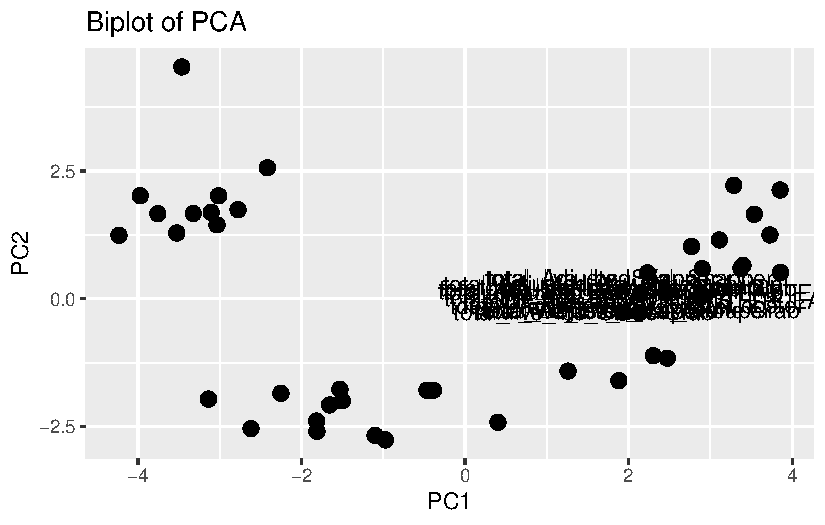
\includegraphics{PCA_all_data_files/figure-pdf/unnamed-chunk-7-1.pdf}

}

\end{figure}

\begin{Shaded}
\begin{Highlighting}[]
\CommentTok{\# Display the biplot}
\FunctionTok{print}\NormalTok{(biplot2)}
\end{Highlighting}
\end{Shaded}

\begin{figure}[H]

{\centering 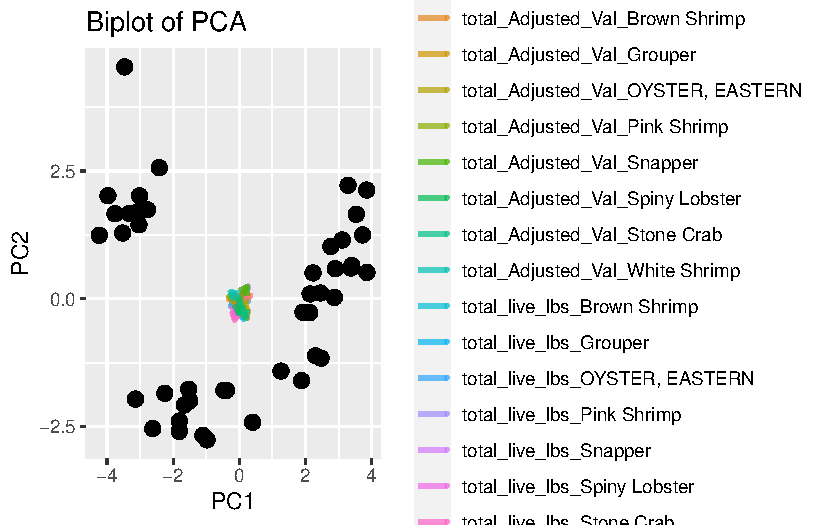
\includegraphics{PCA_all_data_files/figure-pdf/unnamed-chunk-7-2.pdf}

}

\end{figure}

\hypertarget{filter-species-based-on-loadings}{%
\subsubsection{Filter Species based on
loadings}\label{filter-species-based-on-loadings}}

\hypertarget{interpretation}{%
\subsection{Interpretation:}\label{interpretation}}

Species with positive loadings on PC1 based on Values are: Snapper, Blue
Crab, eastern Oyster, Stone crab and Groupeer Species with positive
loadings on PC1 based on Pounds are: Snapper, White Shrimp, Eastern
Oyster and Grouper

==\textgreater{} these are the species that contribute to an increase in
overall variance. Higher values of Snapper, Blue Crab, oyster and
grouper are associated with a positive direction of PC1.

Species with negative loadings on PC1 based on Values: White Shrimp,
Pink Shrmp, Brown Shrimp, Spiny Lobster Species with negative Loadings
on PC1 based on pounds: Pink Shrimp, Brown Shrimp, Spiny Lobster, Stone
Crab

\begin{Shaded}
\begin{Highlighting}[]
\CommentTok{\# Assuming pca\_result is your PCA result}
\NormalTok{loadings }\OtherTok{\textless{}{-}}\NormalTok{ pca\_result}\SpecialCharTok{$}\NormalTok{rotation}

\CommentTok{\# Extract loadings for PC1 and PC2}
\NormalTok{loadings\_PC1 }\OtherTok{\textless{}{-}}\NormalTok{ loadings[, }\DecValTok{1}\NormalTok{]}
\NormalTok{loadings\_PC2 }\OtherTok{\textless{}{-}}\NormalTok{ loadings[, }\DecValTok{2}\NormalTok{]}

\CommentTok{\# Create a data frame with species and their loadings on PC1 and PC2}
\NormalTok{loadings\_data }\OtherTok{\textless{}{-}} \FunctionTok{data.frame}\NormalTok{(}\AttributeTok{species =} \FunctionTok{rownames}\NormalTok{(loadings), }\AttributeTok{PC1 =}\NormalTok{ loadings\_PC1, }\AttributeTok{PC2 =}\NormalTok{ loadings\_PC2)}

\CommentTok{\# Create separate plots for positive and negative loadings on PC1 and PC2}
\FunctionTok{library}\NormalTok{(ggplot2)}

\CommentTok{\# Plot for positive loadings on PC1}
\FunctionTok{ggplot}\NormalTok{(}\FunctionTok{subset}\NormalTok{(loadings\_data, PC1 }\SpecialCharTok{\textgreater{}} \DecValTok{0}\NormalTok{), }\FunctionTok{aes}\NormalTok{(}\AttributeTok{x =}\NormalTok{ PC1, }\AttributeTok{y =}\NormalTok{ PC2, }\AttributeTok{label =}\NormalTok{ species)) }\SpecialCharTok{+}
  \FunctionTok{geom\_text}\NormalTok{() }\SpecialCharTok{+}
  \FunctionTok{ggtitle}\NormalTok{(}\StringTok{"Species with Positive Loadings on PC1"}\NormalTok{)}
\end{Highlighting}
\end{Shaded}

\begin{figure}[H]

{\centering 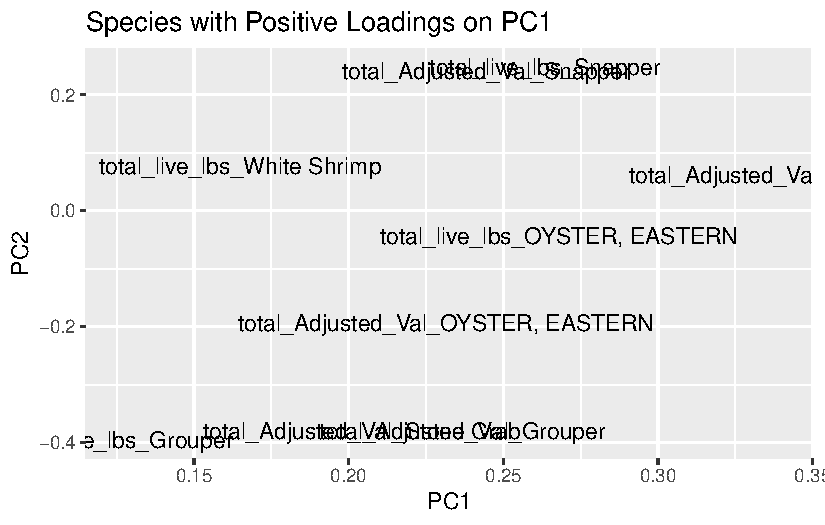
\includegraphics{PCA_all_data_files/figure-pdf/unnamed-chunk-8-1.pdf}

}

\end{figure}

\begin{Shaded}
\begin{Highlighting}[]
\CommentTok{\# Plot for negative loadings on PC1}
\FunctionTok{ggplot}\NormalTok{(}\FunctionTok{subset}\NormalTok{(loadings\_data, PC1 }\SpecialCharTok{\textless{}} \DecValTok{0}\NormalTok{), }\FunctionTok{aes}\NormalTok{(}\AttributeTok{x =}\NormalTok{ PC1, }\AttributeTok{y =}\NormalTok{ PC2, }\AttributeTok{label =}\NormalTok{ species)) }\SpecialCharTok{+}
  \FunctionTok{geom\_text}\NormalTok{() }\SpecialCharTok{+}
  \FunctionTok{ggtitle}\NormalTok{(}\StringTok{"Species with Negative Loadings on PC1"}\NormalTok{)}
\end{Highlighting}
\end{Shaded}

\begin{figure}[H]

{\centering 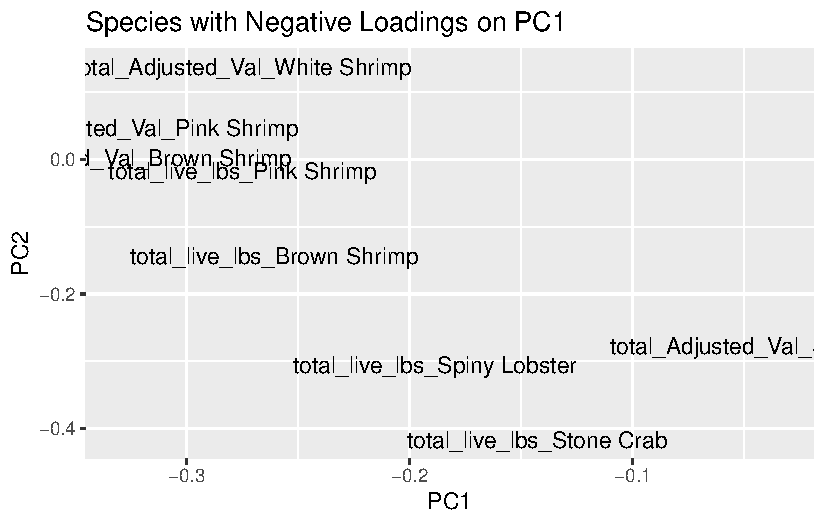
\includegraphics{PCA_all_data_files/figure-pdf/unnamed-chunk-8-2.pdf}

}

\end{figure}

\begin{Shaded}
\begin{Highlighting}[]
\CommentTok{\# Plot for positive loadings on PC2}
\FunctionTok{ggplot}\NormalTok{(}\FunctionTok{subset}\NormalTok{(loadings\_data, PC2 }\SpecialCharTok{\textgreater{}} \DecValTok{0}\NormalTok{), }\FunctionTok{aes}\NormalTok{(}\AttributeTok{x =}\NormalTok{ PC1, }\AttributeTok{y =}\NormalTok{ PC2, }\AttributeTok{label =}\NormalTok{ species)) }\SpecialCharTok{+}
  \FunctionTok{geom\_text}\NormalTok{() }\SpecialCharTok{+}
  \FunctionTok{ggtitle}\NormalTok{(}\StringTok{"Species with Positive Loadings on PC2"}\NormalTok{)}
\end{Highlighting}
\end{Shaded}

\begin{figure}[H]

{\centering 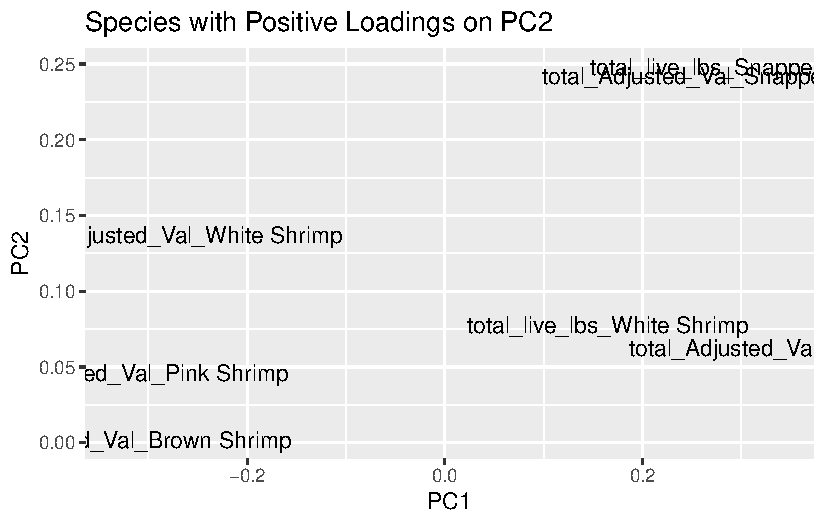
\includegraphics{PCA_all_data_files/figure-pdf/unnamed-chunk-8-3.pdf}

}

\end{figure}

\begin{Shaded}
\begin{Highlighting}[]
\CommentTok{\# Plot for negative loadings on PC2}
\FunctionTok{ggplot}\NormalTok{(}\FunctionTok{subset}\NormalTok{(loadings\_data, PC2 }\SpecialCharTok{\textless{}} \DecValTok{0}\NormalTok{), }\FunctionTok{aes}\NormalTok{(}\AttributeTok{x =}\NormalTok{ PC1, }\AttributeTok{y =}\NormalTok{ PC2, }\AttributeTok{label =}\NormalTok{ species)) }\SpecialCharTok{+}
  \FunctionTok{geom\_text}\NormalTok{() }\SpecialCharTok{+}
  \FunctionTok{ggtitle}\NormalTok{(}\StringTok{"Species with Negative Loadings on PC2"}\NormalTok{)}
\end{Highlighting}
\end{Shaded}

\begin{figure}[H]

{\centering 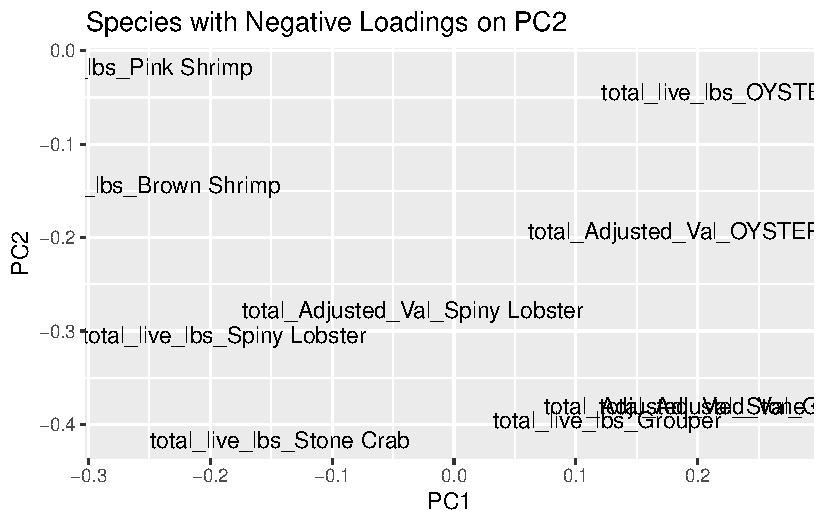
\includegraphics{PCA_all_data_files/figure-pdf/unnamed-chunk-8-4.pdf}

}

\end{figure}



\end{document}
